\documentclass{article}
\usepackage{biblatex}
\usepackage{graphicx}
\usepackage{float}
\addbibresource{prosem.bib}
\begin{document}
\section{Non-Linear Filters}
Non-linear filters serve as additional ways of filtering images. Linear filters can work exceptionally well for certain cases, however one will encounter scenarios where using Non-Linear filters will lead to a better result both visually (Image Processing) and performance-wise. One example noise removal, but more on that later. First of all it is important to look at what non-linear filters actually are.

\subsection{What are Non-Linear Filters?}
First and foremost, what are Non-Linear filters? As mentioned previously, linear filters are filters where the signal-response of two signals and the sum of the responses to the two signals individually are the same. Based on that one may probably guess that non-linear filters are filters where this criteria is not satisfied, and this is the case. This could mean that, in relation to the input data, the transformation could, for instance, be exponential as opposed to linear. This can lead to bigger difficulties concerning frequency response analysis,\cite[p.~132]{szeliski} shift-invariance, etc.
\subsection{Some different types of Non-Linear filters}
\subsubsection{Median Filtering}
Consider a scenario with so-called salt and pepper noise, i.e. an image with noise consisting of sporadic black and white pixels. Were one to use for instance a Gaussian filter, one would quickly end up with a slightly blurred version of the original image. The noise would most likely still be there, simply in a slightly blurred format. Somewhat of a disappointment. There are however other methods of filtering, and for this scenario, a median filter would most likely do the trick.

\begin{figure}[H]
    \centering
    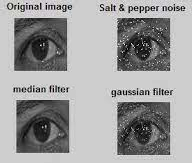
\includegraphics[width=0.5\linewidth]{medianfiltering.jpeg}
    \caption{The same image processed with a median filter and a Gaussian filter. Both filters remove salt and pepper noise (in varying degrees) and produce a result that more accurately corresponds with how the image should look without noise}
    \label{fig:enter-label} 
\end{figure}
Now we have seen an example median filtering, compared to Gaussian filtering, for a specific scenario, and what it does, it is time to dive into what a \textit{median filter actually is}. The algorithm works in this way: Given an input signal, in this case an image, it goes through every single pixel of the image, and replaces the value with the median value of the adjacent pixels. One can also let it go through the image whilst checking adjacent pixels in a 3px, 10px, or generally X-pixel radius around the current one, and replace it with the median of the pixels inside this X-pixel radius. The "X-pixel radius" is called a kernel. Increasing the kernel-size of the filter might lead to a "smeared" and somewhat blurry look in many scenarios.
\begin{figure}{h}
    \centering
    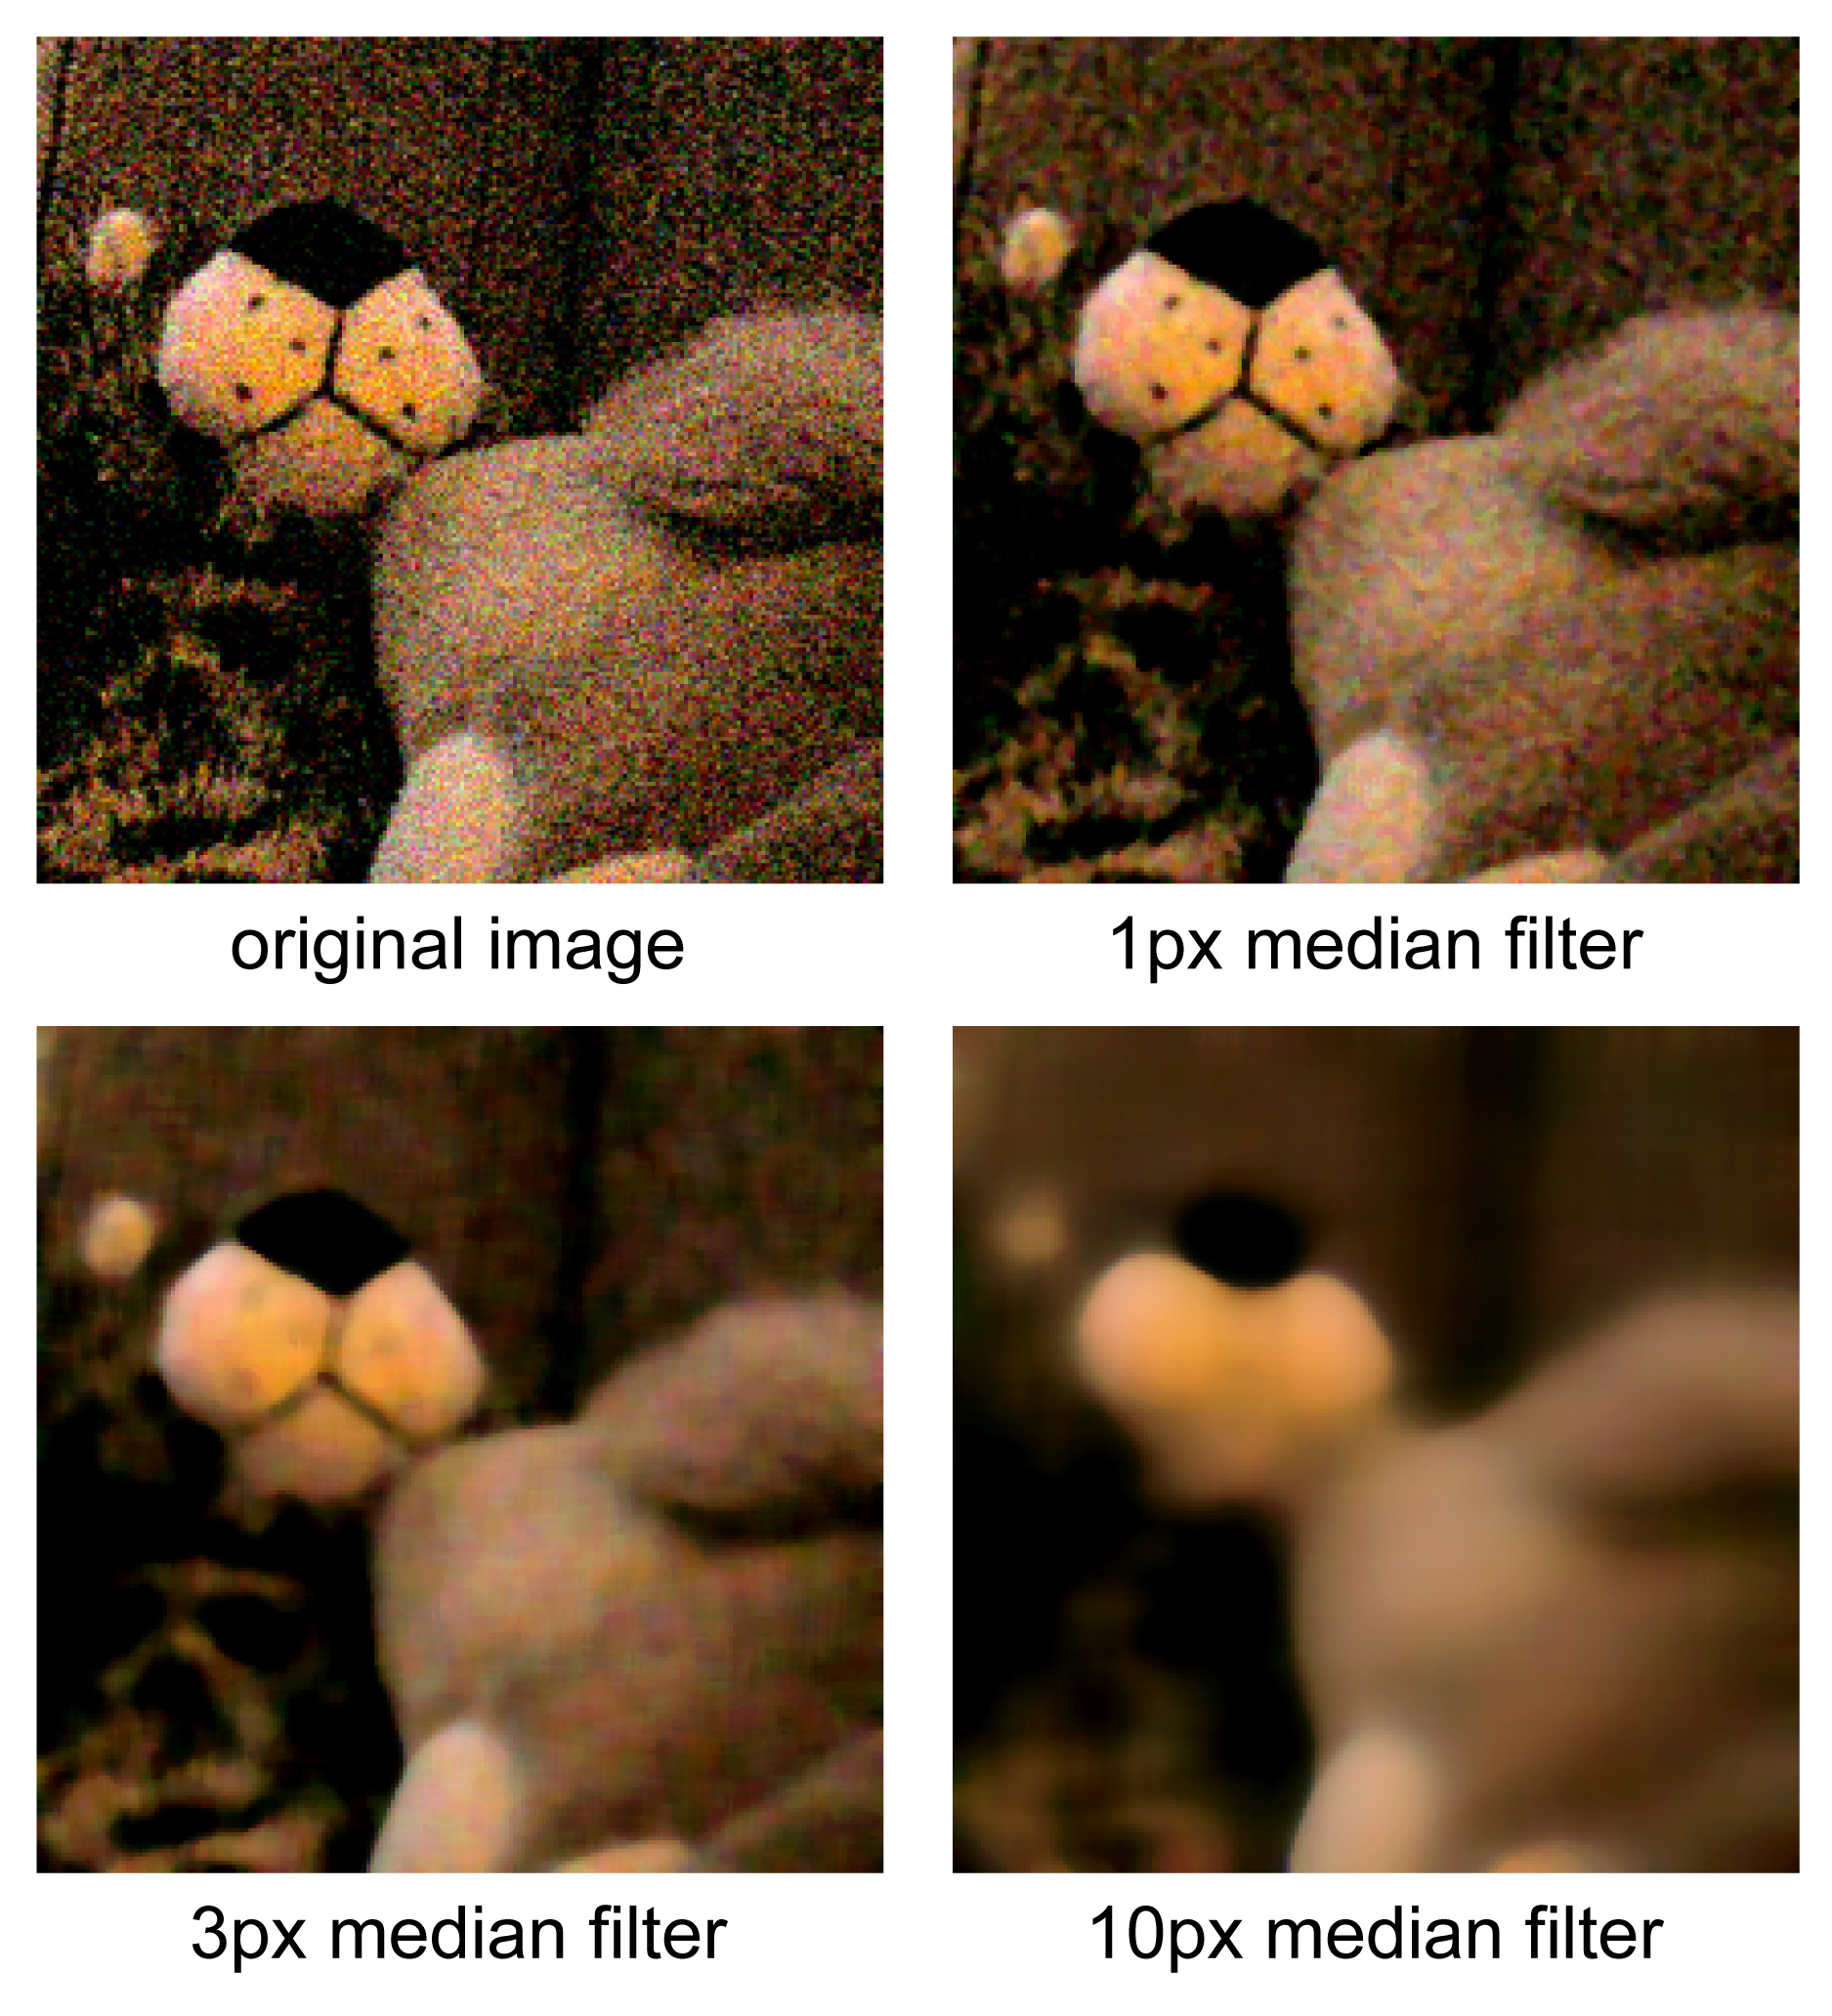
\includegraphics[width=0.5\linewidth]{median_example.jpg}
    \caption{Processing the image with a bigger kernel radius leads to less "crispness"}
    \label{fig:enter-label}
\end{figure}
\begin{figure}{h}
    \centering
    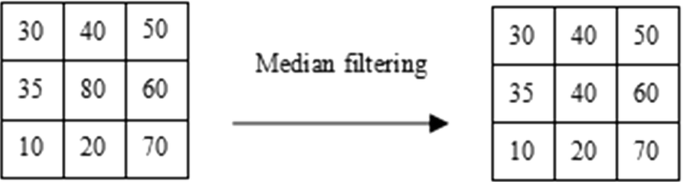
\includegraphics[width=0.5\linewidth]{medianfiltering.PNG}
    \caption{lllustration of how the mean filter algorithm works. The central pixel's value is changed from 80 to 40. 40 is the median of all the values within a 1px radius of the central pixel.}
    \label{fig:enter-label}
\end{figure}
However, even though median filters work relatively well for this specific scenario, the cure for cancer is yet to be found. There are (several) scenarios in which median filters might produce sub-optimal results.

\subsubsection{Bilateral Filtering}
Another type of Non-Linear filter is the bilateral filter. In order to properly understand the bilateral filter, it is first important to understand a few other principles.

It would, at this point, be prudent to mention a certain property of filters that can be very much sought after, namely, \textit{edge-preservation}. When filtering away noise one often runs the risk of losing the clarity of the edges in the image. Given an image with a coin, and some noise, one might filter away the noise with a filter, perhaps a Gaussian would work here. After applying the filter, the noise might have been cleared away, but one will often recognize a certain "smudgyness" by the edges. The, perhaps, once sharp clear edges where the coins meet the background have seemingly melted more into their surroundings. Somewhat problematic. Applying an even stronger filter might remove the clear edge of the coins completely, making the coins look more like the sun in the middle of day than the coins they supposedly are.
\begin{figure}[H]
    \centering
    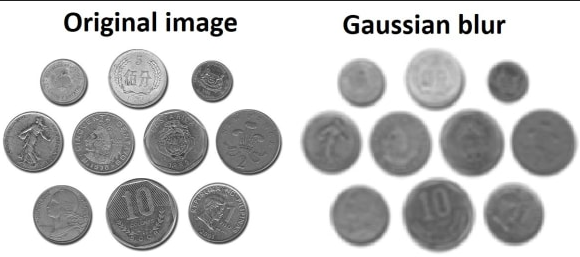
\includegraphics[width=0.5\linewidth]{coins.PNG}
    \caption{Applying a Gaussian-filter has made the edges of the coins less pronounced. This goes for the background-coin-edge, and also the edges of the coin details such as numbers and figures}
    \label{fig:enter-label}
\end{figure}

Another important filtering method to recognize, at this point, is weighted kernel filtering. Weighted kernel filtering is an extension of the median filter. It works by \textit{weighting} pixels based on their distance from the middle. I.e. the further the pixel is from the center, the smaller the effect of it, but importantly, it still has an influence!

Now to bilateral filters themselves. The base principle of bilateral filtering is applying the concept of weighted median filtering, yet with a tweak. The bilateral filter rejects values that are too much of an outlier for the current kernel, hence, often preserving edges better than the previously mentioned filters. Since a median filter uses all pixel-values in the kernel when processing an image, it may very well lead to blurred edges. Imagine, for instance, the aforementioned example with the coins (Figure 3.4). When the median filter does it's magic on the edges, for instance where the coin meets the background, it will use the values of the white background, and mix it into the values of the darker coins edges. Ergo, the edge of the darker coin will turn into a lighter colour because of the influence of the background. Apply the median filter several more times, and this will happen again and again and again, quickly leading to an unrecognizable blur, rather than a crisp clear image of coins with the noise removed (Note: This will most likely happen regardless of filter if one applies it an excessive amount of times, but the amount of times one must apply the filter for the image to become unrecognizably blurry or smudge-like is different).

Let's consider filtering the same image with a bilateral filter. When the bilateral filter considers pixels along the edge of the coins it will not consider outliers, hence, it will not consider the pixels of the strong white background, rather focusing on the pixels of the coin itself, as they are more similar to the relevant pixel. That is not to say that applying the bilateral filter an exorbitant amount of times won't lead to the edges eventually blending into their surroundings, but the bilateral filter does, for most intents and purposes, preserve edges.


\subsubsection{Minimum- and Maximum Filtering}
Two more types of non-linear filters are minimum- and maximum filters. These two filters are often also called dilation and erosion filters, respectively. They are classified amongst the so called morphological filters. In many ways, the minimum and maximum filters are two sides of the same coin, they are very similar in all but one point. As the minimum filter moves along the image, processing as it should, it simply chooses the smallest value inside the current kernel and applies this value to the relevant pixel. Maximum filters work very similarly, but, as one might guess, they instead pick the largest value and assigns that to the relevant pixel. Given the two filters other names, dilation and erosion, it might not be too much of a leap to assume what an image processed by these filters would look like relative to the original. Minimum filters, or dilation filters, simply dilate the darker areas of images (since darker values tend to be assigned lower numbers). Effective if one wishes to thicken the borders of a dark-coloured letter on a light background in an image. Contrarily, the maximum filter, or erosion filter, will erode darker pixels from images. If a black pixel is surrounded by only white pixels, it will be gone after an erosion filter has been applied.
Lastly on minimum and maximum filters, a bit about binary images. What are binary images? They are in fact part of what led to the creation of morphological filters such as the here discussed minimum and maximum ones. As one might deduce from the name "binary images"  they operate with \textit{only} binary values. In other terms, each pixel can only have one of two values, black and white.
\begin{figure}[H]
    \centering
    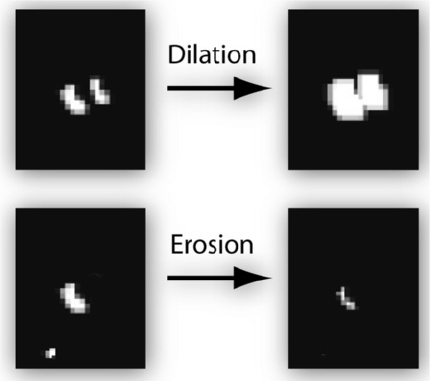
\includegraphics[width=0.5\linewidth]{minmax1.png}
    \caption{Illustrates the usage of minimum and maximum filters on a grayscale image. Using the minimum filter expands the area of the figure, whereas applying a maximum filter reduces it's size}
\end{figure}

\begin{figure}[H]
    \centering
    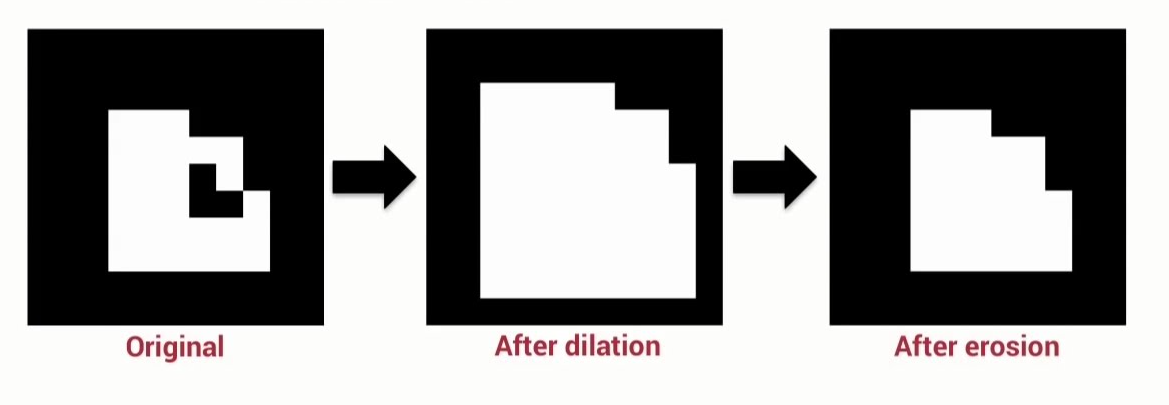
\includegraphics[width=0.5\linewidth]{minmax2.PNG}
    \caption{Illustration of three binary images. Using a minimum filter succeeded by a maximum filter fills the gaps in the figure and then decreases it's size}
    \label{fig:enter-label}
\end{figure}
\subsection{Further Non-Linear filter related techniques}
\subsubsection{Mean Shift}
The mean shift algorithm is often referred to as a "hill climbing algorithm". Given for instance a scatter plot, or such, the mean shift algorithm will locate the area of the plot where the data-point density is at it's highest, metaphorically speaking, a hill (densest data cluster). Roughly, the algorithm will move (shift) from data point to data point based on the regional mean (mean of current cluster). What is considered in calculating the mean may vary from implementation to implementation. Some times calculating a weighted mean may yield more accurate results, depending on what one is searching for.
How can one apply this concept in image processing? Mostly in image segmentation. As mean shift is quite prolific at finding and recognizing clusters, it is also quite good at recognizing "clusters" in images, i.e. different parts of an image. Segmenting an image, categorizing different parts of it, can allow you to perhaps apply different filtering algorithms for different areas of the image, maybe help with edge detection, and in general help preserve the intended look and data of the image. Furthermore it has applications in for instance computer vision and pattern recognition. Important (sub-)fields of image processing.
\begin{figure}[H]
    \centering
    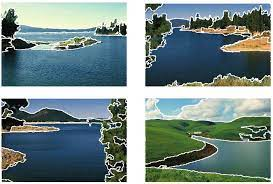
\includegraphics[width=0.5\linewidth]{meanshift.jpeg}
    \caption{Four different images, all segmented by a mean shift algorithm. The segmentation enables one to analyze different areas in different ways. Maybe one would rather filter noise away from water-areas or different coloured areas with different filtering techniques}
    \label{fig:enter-label}
\end{figure}
\begin{figure}[H]
    \centering
    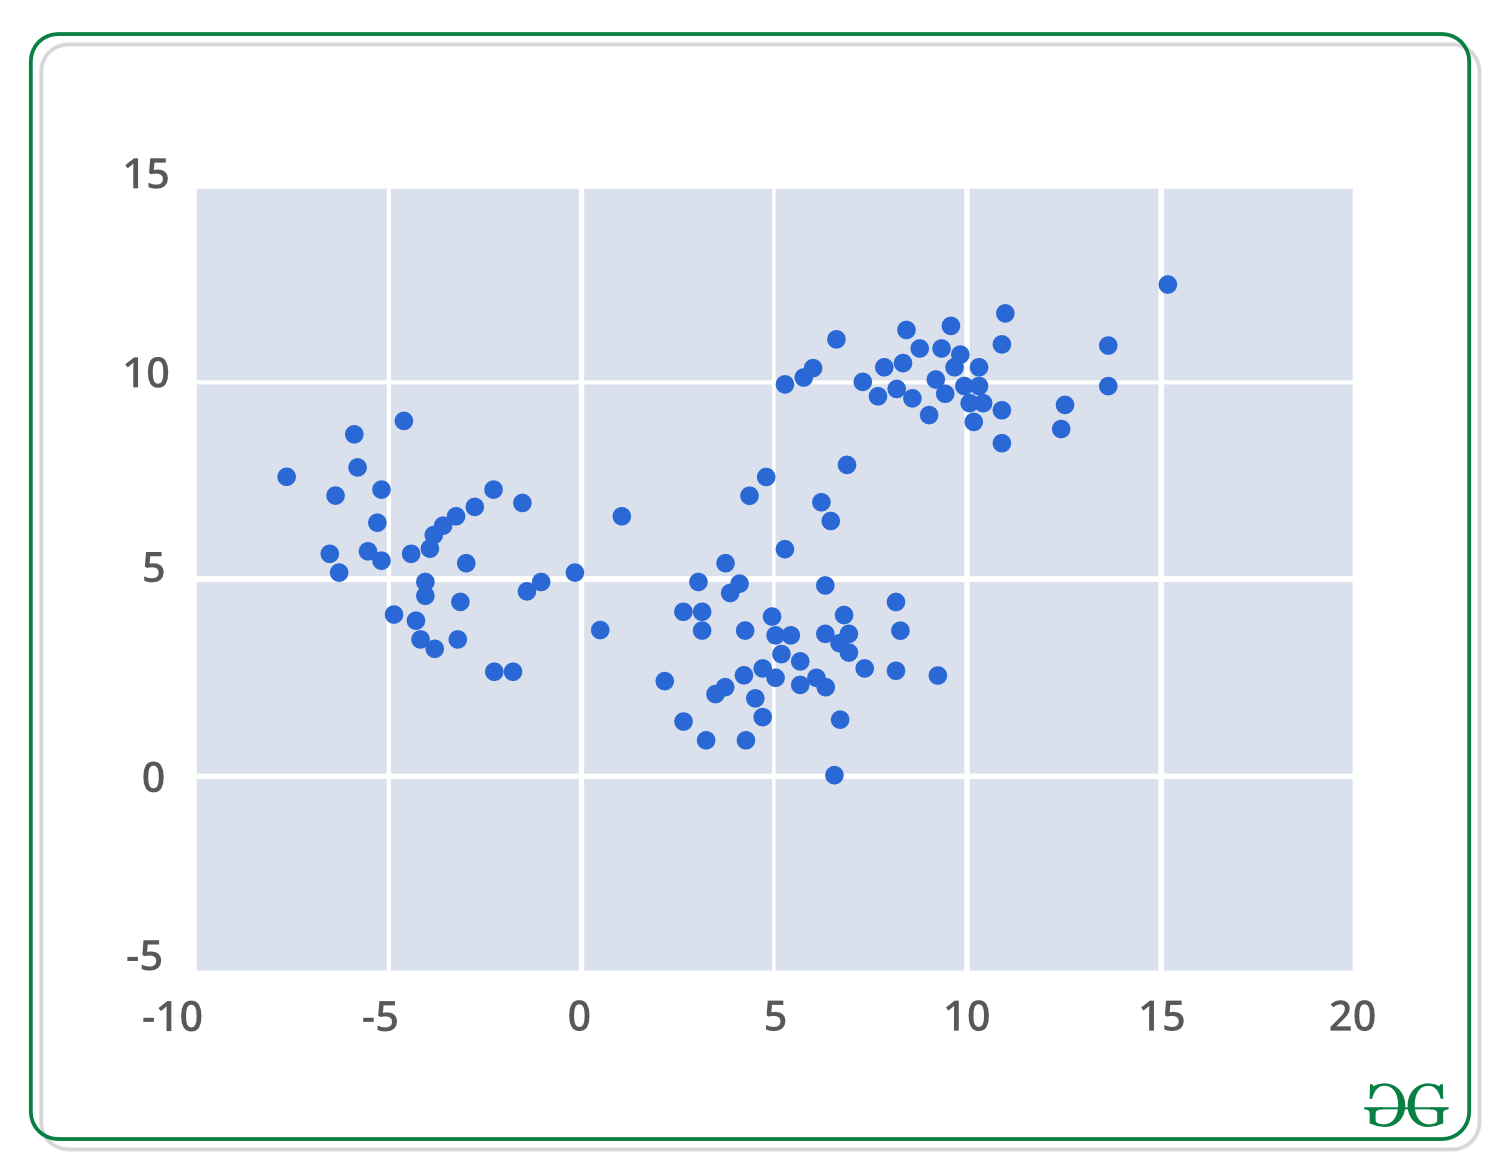
\includegraphics[width=0.5\linewidth]{scattergraph.png}
    \caption{A typical graph for which the mean shift algorithm could be applied. The clusters can be viewed as hills. Increased data point density would imply a "steeper hill". One can roughly recognize the outline of three main clusters here}
    \label{fig:enter-label}
\end{figure}

\subsubsection{Cellular Automata}
Cellular automata is something one probably has heard about in other contexts than image processing. Tracing it roots back to the late 40s, as the brainchild of the two late great scientists Stanislaw Ulam, and of course, the father of computer science himself Neumann Janos, commonly known as John von Neumann. Von Neumann was working on self-replicating-systems when he, with some help from Ulam, came up with his Cellular Automaton. Proving that his self-replicating automaton would work. But how can one apply this seemingly unrelated part of computer science to image processing?  First of all, let's assess how cellular automata work.

In essence, cellular automata are grids of cells, each containing what can be considered a finite state machine. They can be very useful in the analysis of many different systems, as well as in the fields of physics and biology. A famous example/application of cellular automata is Conway's game of life\cite{gardnermathematical}.
Now how specifically does one apply a cellular automaton to image processing?  As of now one of the most major application areas is noise removal in binary images. \cite{inproceedings} As demonstrated by Rosin and Sun\cite{rosin} it can also be used for edge detection, which, as previously mentioned, is an \textit{essential} part of image processing.
\begin{figure}{H}
    \centering
    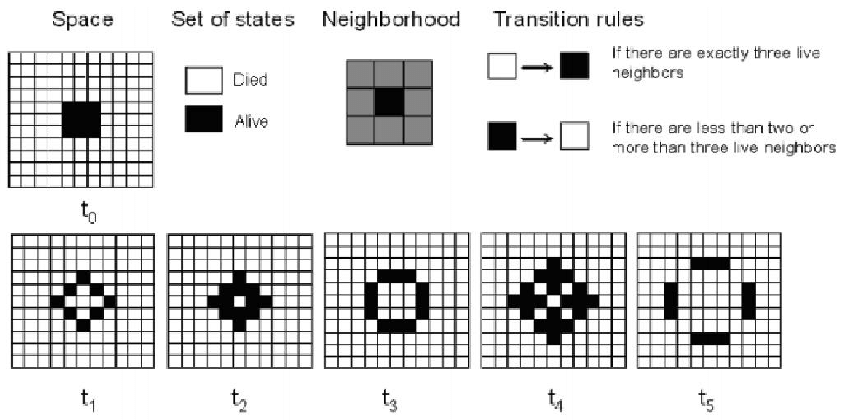
\includegraphics[width=0.5\linewidth]{gameoflife.png}
    \caption{An illustration of Conway's game of life. An important milestone in the study of Cellular Automata, and also a good example of what Cellular Automata can look like}
    \label{fig:enter-label}
\end{figure}
\subsection{Anisotropic Diffusion}
As discussed, there are several scenarios in which non-linear filters can help improve the clarity of images, but sometimes one may actually wish to blur certain areas of an image. Say, for instance, one wishes to recognize the outline of a person, an animal, a car, or similar in an image. Using edge-detection one might well find the edges accurately, but what when the edge-detection algorithm also detects features of the figures as edges, and not only the outline? This is where (anisotropic) diffusion can come into play. Diffusion in general will "smudge out" the image, letting edges and borders flow into one another creating an image where shapes may be hard to distinguish from one another. This is useful, as this is, in a sense, what we wish to do with the "inner details" of the figure we are trying to find the outline of. Still, there is somewhat of a problem remaining, the fact that only diffusing the image will lead to \textit{all} the edges and borders being hard to detect. Where anisotropic diffusion veers of from standard diffusion is by preserving the strongest edges or borders, the outlines. By controlling what is diffused and not, we diffuse only the contents inside the borders, hence making the most prominent edges all the more prominent relative to the rest of the image. This will allow us to figure out the outline of a figure more accurately, as the outline tends to be the most prominent border.
\begin{figure}{H}
    \centering
    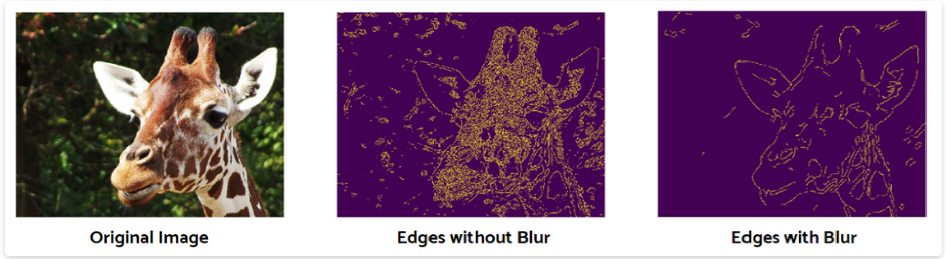
\includegraphics[width=1\linewidth]{edgedetection.png}
    \caption{Filtering can be a double edged-sword. Depending on what data one is searching for, one may not need to preserve every single edge in an image. For this scenario, if one is trying to recognize a clear outline of the giraffe, it is easier to find in a blurred version of the image}
    \label{fig:enter-label}
\end{figure}

\subsection{Typical applications of Non-Linear filters}
The subject of where one can apply Non-Linear filters has already been touched upon. Likely, the most prominent application area of non-linear filters in image processing is in noise filtering. Filtering away noise can be invaluable for increasing the clarity of a given image. A further application of non-linear filters is edge detection. Edge detection can be of vital importance (quite literally) in image processing, especially when applied in the context of computer vision, and for instance, autonomous cars. Non-Linear filters may also help in image enhancement and restoration, mostly through aforementioned applications such as noise-removal, pattern recognition (edge detection/segementation) and further techniques such as increasing contrast. Image restoration and enhancement can even be used to increase the resolution (upscaling) of images and videos, allowing old films to be re-released in higher resolutions. From the old graininess of VHS to HD and full HD all the way to UHD and 4k/8k resolutions. This process is of course not magic though, and it cannot create something that does not exist, hence it also cannot recover completely lost information\cite{sharmila}
\begin{figure}{H}
    \centering
    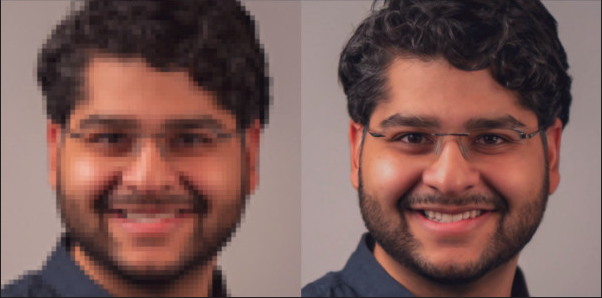
\includegraphics[width=1\linewidth]{upscaling.PNG}
    \caption{Non-Linear filtering can be a vital component in image enhancement and upscaling. In this photo the image has been upscaled from 64x64 to an impressive 1024x1024}
    \label{fig:enter-label}
\end{figure}

\subsection{Conclusion}
Now that we have discussed some different image processing algorithms, specifically several linear and non-linear filtering ones it is time to assess their use cases, and to compare them. A first obvious question that may arise is whether any specific type of filtering is simply objectively better. As with many situations in life, and different fields of computer science, this is hard to find. Just as it may be hard to determine a specific sorting algorithm as objectively the best in any given scenario, it is equally hard to determine an objectively best filtering algorithm. In some programs or prototypes it may be prudent to apply a simple filtering algorithm as nothing too extensive is needed. For ease of use and understanding, many linear filters may well hold the edge over most non-linear filters. Many non-linear filters can seem less intuitive, and hence be harder to understand and implement, possibly being overly complex for certain scenarios. It is also important to note that in most use cases, be that in pure image processing, signal processing or computer vision, many filters are used in combination to achieve optimal results. Applying specific filtering techniques for specific scenarios and then weaving all the data they produce together may well produce far more accurate data than taking a "one-size fits all" approach to filters.

Filtering can be an incredibly helpful tool in processing images. Removing noise from images, increasing clarity, detecting edges and such have applications in the closely related field of computer vision as well, but none of this comes without it's drawbacks. As we have seen, applying a wrong filter can easily lead to a decrease in clarity of images, perhaps only succeeding in making an image more blurry. Moreover, even if applying "the optimal" filtering algorithm it by no stretch of the imagination guarantees a completely noise and error free result. Filtering is not magic, certain images may be past a point in which it physically cannot get any clearer. This also leads into another issue, namely over-processing. Passing a signal or an image through a filter one time (or more) too many can lead to results which no longer resemble the original, what it was supposed too look like, or lead to unnatural results. In these cases, one may very well consider whether the application of a filter actually helped. If one in certain scenarios realizes that the answer for this case was actually no, one may already have spent far too many resources and hours on something that ended up being producing nothing practical. Resource management is very often of the essence.

Even with all the potential drawbacks that filtering can bring, the pros most likely heavily outweigh the cons. As technology advances, new techniques and new equipment will lead to even more advanced image processing. With the advent of AI, many of it's techniques may be appended to already existing techniques, or spawn new ones entirely. This will all surely lead to even more advanced filtering techniques, and with the blistering increase of data (big data) out there, there is no lack in training data for all AI/ML/Neural Network's needs. This will probably be the most major source of improvement for future filtering techniques. Another important area of improvement is efficiency. Increased hardware performance will lead to faster filtering algorithms working even more efficiently. Further research, and development of the algorithms will also lead to a better (lower) time-complexity, hence increasing the filtering algorithms efficiency further. This is of the utmost importance in, for instance, computer vision for autonomous cars. Faster processing and filtering of the image data a self-driving car collects can be the difference between life and death, and can drastically improve the safety of these self-driving cars.

\printbibliography

\end{document}